\chapter{Results}

% This chapter contains the results of our analysis of the data that we collected through the methods outlined in Chapter 3. We first analyze the number of students who fell under each attendance type as determined by their responses to the surveys and the online attendance metrics. From there, we describe the responses that we received from survey and interview participants. Finally, we provide an overview for what we determined to be the biggest factors that impacted students' decision-making prior to and during their enrollment in the course.

\section{Attendance Across Modalities}

\subsection{Types of Attendance}

\begin{table}[H]
    \centering
    \captionsetup{justification=centering}
    \caption{Percentages of respondents who attended lectures through each modality in the first and second half of the course}
    \begin{tabular}{|c|cccc|c|c|}
        \hline
        \rowcolor[HTML]{B7B7B7} 
        \cellcolor[HTML]{B7B7B7}                                    & \multicolumn{4}{c|}{\cellcolor[HTML]{B7B7B7}\textbf{Synchronous}}                                                                                                                                                                                                                                           & \cellcolor[HTML]{B7B7B7}                                   & \cellcolor[HTML]{B7B7B7}                                      \\ \cline{2-5}
        \rowcolor[HTML]{B7B7B7} 
        \multirow{-2}{*}{\cellcolor[HTML]{B7B7B7}\textbf{Weeks}}    & \multicolumn{1}{c|}{\cellcolor[HTML]{B7B7B7}\textbf{Hybrid}}                  & \multicolumn{1}{c|}{\cellcolor[HTML]{B7B7B7}\textbf{In-Person}}                & \multicolumn{1}{c|}{\cellcolor[HTML]{B7B7B7}\textbf{Remote}}                   & \textbf{Total}                                            & \multirow{-2}{*}{\cellcolor[HTML]{B7B7B7}\textbf{Async.}}  & \multirow{-2}{*}{\cellcolor[HTML]{B7B7B7}\textbf{No Attend.}} \\ \hline
        \begin{tabular}[c]{@{}c@{}}1 to 5\\ (N = 144)\end{tabular}  & \multicolumn{1}{c|}{\begin{tabular}[c]{@{}c@{}}8.3\%\\ (N = 12)\end{tabular}} & \multicolumn{1}{c|}{\begin{tabular}[c]{@{}c@{}}20.1\%\\ (N = 29)\end{tabular}} & \multicolumn{1}{c|}{\begin{tabular}[c]{@{}c@{}}20.1\%\\ (N = 29)\end{tabular}} & \begin{tabular}[c]{@{}c@{}}48.6\%\\ (N = 70)\end{tabular} & \begin{tabular}[c]{@{}c@{}}42.4\%\\ (N = 61)\end{tabular}  & \begin{tabular}[c]{@{}c@{}}9.0\%\\ (N = 13)\end{tabular}      \\ \hline
        \begin{tabular}[c]{@{}c@{}}6 to 10\\ (N = 232)\end{tabular} & \multicolumn{1}{c|}{\begin{tabular}[c]{@{}c@{}}3.9\%\\ (N = 9)\end{tabular}}  & \multicolumn{1}{c|}{\begin{tabular}[c]{@{}c@{}}12.9\%\\ (N = 30)\end{tabular}} & \multicolumn{1}{c|}{\begin{tabular}[c]{@{}c@{}}8.2\%\\ (N = 19)\end{tabular}}  & \begin{tabular}[c]{@{}c@{}}25.0\%\\ (N = 58)\end{tabular} & \begin{tabular}[c]{@{}c@{}}62.1\%\\ (N = 144)\end{tabular} & \begin{tabular}[c]{@{}c@{}}12.9\%\\ (N = 30)\end{tabular}     \\ \hline
    \end{tabular}
    \label{tab:attendance-modalities-tab}
\end{table}

As can be seen in Table \ref{tab:attendance-modalities-tab}, synchronous attendance was relatively high during the first half of the course, with the mid-course survey data identifying more synchronous attendees than asynchronous attendees. However, the second half of the course saw a decrease in synchronous attendance from approximately half of the student body to a quarter. Within the hybrid and remote classifications, attendance dropped by over 50\%; however, in-person attendance dropped less than proportionally with the other synchronous classifications, dropping by roughly 35\%. In most of the courses that are offered by the department, attendance decreases as students spend more time enrolled, so this was not an unexpected occurrence. Nevertheless, the fact that non-attendees only rose by 3.9\% during the second half of the course indicates that many of the students who stopped attending lectures synchronously continued to attend them through the asynchronous recordings.

\begin{table}[H]
    \vspace{5mm}
    \centering
    \captionsetup{justification=centering}
    \caption{Percentage of students in each modality of attendance, grouped by their preferred modality on the pre-course survey}
    \begin{tabular}{|c|c|cccc|c|c|}
        \hline
        \rowcolor[HTML]{B7B7B7} 
        \cellcolor[HTML]{B7B7B7}                                    & \cellcolor[HTML]{B7B7B7}                                                                                         & \multicolumn{4}{c|}{\cellcolor[HTML]{B7B7B7}\textbf{Synchronous}}                                                                                                                                                                                                                                                                                                                  & \cellcolor[HTML]{B7B7B7}                                  & \cellcolor[HTML]{B7B7B7}                                      \\ \cline{3-6}
        \rowcolor[HTML]{B7B7B7} 
        \multirow{-2}{*}{\cellcolor[HTML]{B7B7B7}\textbf{Weeks}}    & \multirow{-2}{*}{\cellcolor[HTML]{B7B7B7}\textbf{\begin{tabular}[c]{@{}c@{}}Modality\\ Preference\end{tabular}}} & \multicolumn{1}{c|}{\cellcolor[HTML]{B7B7B7}\textbf{Hybrid}}                                          & \multicolumn{1}{c|}{\cellcolor[HTML]{B7B7B7}\textbf{In-Person}}                                        & \multicolumn{1}{c|}{\cellcolor[HTML]{B7B7B7}\textbf{Remote}}                                          & \textbf{Total}                                            & \multirow{-2}{*}{\cellcolor[HTML]{B7B7B7}\textbf{Async.}} & \multirow{-2}{*}{\cellcolor[HTML]{B7B7B7}\textbf{No Attend.}} \\ \hline
                                                                    & \begin{tabular}[c]{@{}c@{}}In-Person\\ (N = 51)\end{tabular}                                                     & \multicolumn{1}{c|}{\begin{tabular}[c]{@{}c@{}}9.8\%\\ (N = 5)\end{tabular}}                          & \multicolumn{1}{c|}{\begin{tabular}[c]{@{}c@{}}41.2\%\\ (N = 21)\end{tabular}}                         & \multicolumn{1}{c|}{\begin{tabular}[c]{@{}c@{}}19.6\%\\ (N = 10)\end{tabular}}                        & \begin{tabular}[c]{@{}c@{}}70.6\%\\ (N = 36)\end{tabular} & \begin{tabular}[c]{@{}c@{}}25.5\%\\ (N = 13)\end{tabular} & \begin{tabular}[c]{@{}c@{}}3.9\%\\ (N = 2)\end{tabular}       \\ \cline{2-8} 
        \begin{tabular}[c]{@{}c@{}}1 to 5\\ (N = 120)\end{tabular}  & \begin{tabular}[c]{@{}c@{}}Remote\\ (N = 41)\end{tabular}                                                        & \multicolumn{1}{c|}{\begin{tabular}[c]{@{}c@{}}9.8\%\\ (N = 4)\end{tabular}}                          & \multicolumn{1}{c|}{\begin{tabular}[c]{@{}c@{}}2.4\%\\ (N = 1)\end{tabular}}                           & \multicolumn{1}{c|}{\begin{tabular}[c]{@{}c@{}}29.3\%\\ (N = 12)\end{tabular}}                        & \begin{tabular}[c]{@{}c@{}}41.5\%\\ (N = 17)\end{tabular} & \begin{tabular}[c]{@{}c@{}}41.5\%\\ (N = 17)\end{tabular} & \begin{tabular}[c]{@{}c@{}}17.1\%\\ (N = 7)\end{tabular}      \\ \cline{2-8} 
                                                                    & \begin{tabular}[c]{@{}c@{}}Either\\ (N = 28)\end{tabular}                                                        & \multicolumn{1}{c|}{\begin{tabular}[c]{@{}c@{}}3.6\%\\ (N = 1)\end{tabular}}                          & \multicolumn{1}{c|}{\begin{tabular}[c]{@{}c@{}}10.7\%\\ (N = 3)\end{tabular}}                          & \multicolumn{1}{c|}{\begin{tabular}[c]{@{}c@{}}3.6\%\\ (N = 1)\end{tabular}}                          & \begin{tabular}[c]{@{}c@{}}17.9\%\\ (N = 5)\end{tabular}  & \begin{tabular}[c]{@{}c@{}}67.9\%\\ (N = 19)\end{tabular} & \begin{tabular}[c]{@{}c@{}}14.3\%\\ (N = 4)\end{tabular}      \\ \hline
        \rowcolor[HTML]{D9D9D9} 
                                                                    & \begin{tabular}[c]{@{}c@{}}In-Person\\ (N = 59)\end{tabular}                                                     & \multicolumn{1}{c|}{\cellcolor[HTML]{D9D9D9}\begin{tabular}[c]{@{}c@{}}11.9\%\\ (N = 7)\end{tabular}} & \multicolumn{1}{c|}{\cellcolor[HTML]{D9D9D9}\begin{tabular}[c]{@{}c@{}}23.7\%\\ (N = 14)\end{tabular}} & \multicolumn{1}{c|}{\cellcolor[HTML]{D9D9D9}\begin{tabular}[c]{@{}c@{}}11.9\%\\ (N = 7)\end{tabular}} & \begin{tabular}[c]{@{}c@{}}47.5\%\\ (N = 28)\end{tabular} & \begin{tabular}[c]{@{}c@{}}44.1\%\\ (N = 26)\end{tabular} & \begin{tabular}[c]{@{}c@{}}8.5\%\\ (N = 5)\end{tabular}       \\ \cline{2-8} 
        \rowcolor[HTML]{D9D9D9} 
        \begin{tabular}[c]{@{}c@{}}6 to 10\\ (N = 165)\end{tabular} & \begin{tabular}[c]{@{}c@{}}Remote\\ (N = 65)\end{tabular}                                                        & \multicolumn{1}{c|}{\cellcolor[HTML]{D9D9D9}\begin{tabular}[c]{@{}c@{}}1.5\%\\ (N = 1)\end{tabular}}  & \multicolumn{1}{c|}{\cellcolor[HTML]{D9D9D9}\begin{tabular}[c]{@{}c@{}}6.2\%\\ (N = 4)\end{tabular}}   & \multicolumn{1}{c|}{\cellcolor[HTML]{D9D9D9}\begin{tabular}[c]{@{}c@{}}6.2\%\\ (N = 4)\end{tabular}}  & \begin{tabular}[c]{@{}c@{}}13.8\%\\ (N = 9)\end{tabular}  & \begin{tabular}[c]{@{}c@{}}72.3\%\\ (N = 47)\end{tabular} & \begin{tabular}[c]{@{}c@{}}13.8\%\\ (N = 9)\end{tabular}      \\ \cline{2-8} 
        \rowcolor[HTML]{D9D9D9} 
                                                                    & \begin{tabular}[c]{@{}c@{}}Either\\ (N = 41)\end{tabular}                                                        & \multicolumn{1}{c|}{\cellcolor[HTML]{D9D9D9}\begin{tabular}[c]{@{}c@{}}0.0\%\\ (N = 0)\end{tabular}}  & \multicolumn{1}{c|}{\cellcolor[HTML]{D9D9D9}\begin{tabular}[c]{@{}c@{}}9.8\%\\ (N = 4)\end{tabular}}   & \multicolumn{1}{c|}{\cellcolor[HTML]{D9D9D9}\begin{tabular}[c]{@{}c@{}}12.2\%\\ (N = 5)\end{tabular}} & \begin{tabular}[c]{@{}c@{}}22.0\%\\ (N = 9)\end{tabular}  & \begin{tabular}[c]{@{}c@{}}56.1\%\\ (N = 23)\end{tabular} & \begin{tabular}[c]{@{}c@{}}22.0\%\\ (N = 9)\end{tabular}      \\ \hline
    \end{tabular}
    \label{tab:attendance-initial-preference}
\end{table}

In addition, when we stratify the students of each attendance type by their stated modality of preference on the pre-course survey, we can hypothesize that there exists a relationship between the two: as seen in Table \ref{tab:attendance-initial-preference}, students who stated that they preferred in-person instruction were much more likely to attend in person during the first half of the course, with 41.2\% of those who preferred in-person attending lectures in person compared to 2.4\% of those who preferred remote and 10.7\% of those who stated no preference between the two. In contrast, students who preferred remote or had no preference were much more likely to attend lectures asynchronously at 41.5\% and 67.9\%, respectively, compared to 25.5\% of those who preferred in-person.

The second half of the course saw a shift away from synchronous attendance in favor of asynchronous and non-attendance across all preference types, but the students who preferred in-person still made up the majority of in-person attendance during that period. Students who preferred remote had the largest shift to asynchronous attendance of the three preference types, with 72.3\% attending asynchronously compared to 41.5\% in the first half of the course. We also found that, unlike the other two preference types, the proportion of non-attendees among students who preferred remote fell from 17.1\% in the first half of the course to 13.8\% in the second half.

\subsection{Synchronous Attendance Over Time}

\begin{figure}[H]
    \vspace{5mm}
    \centering
    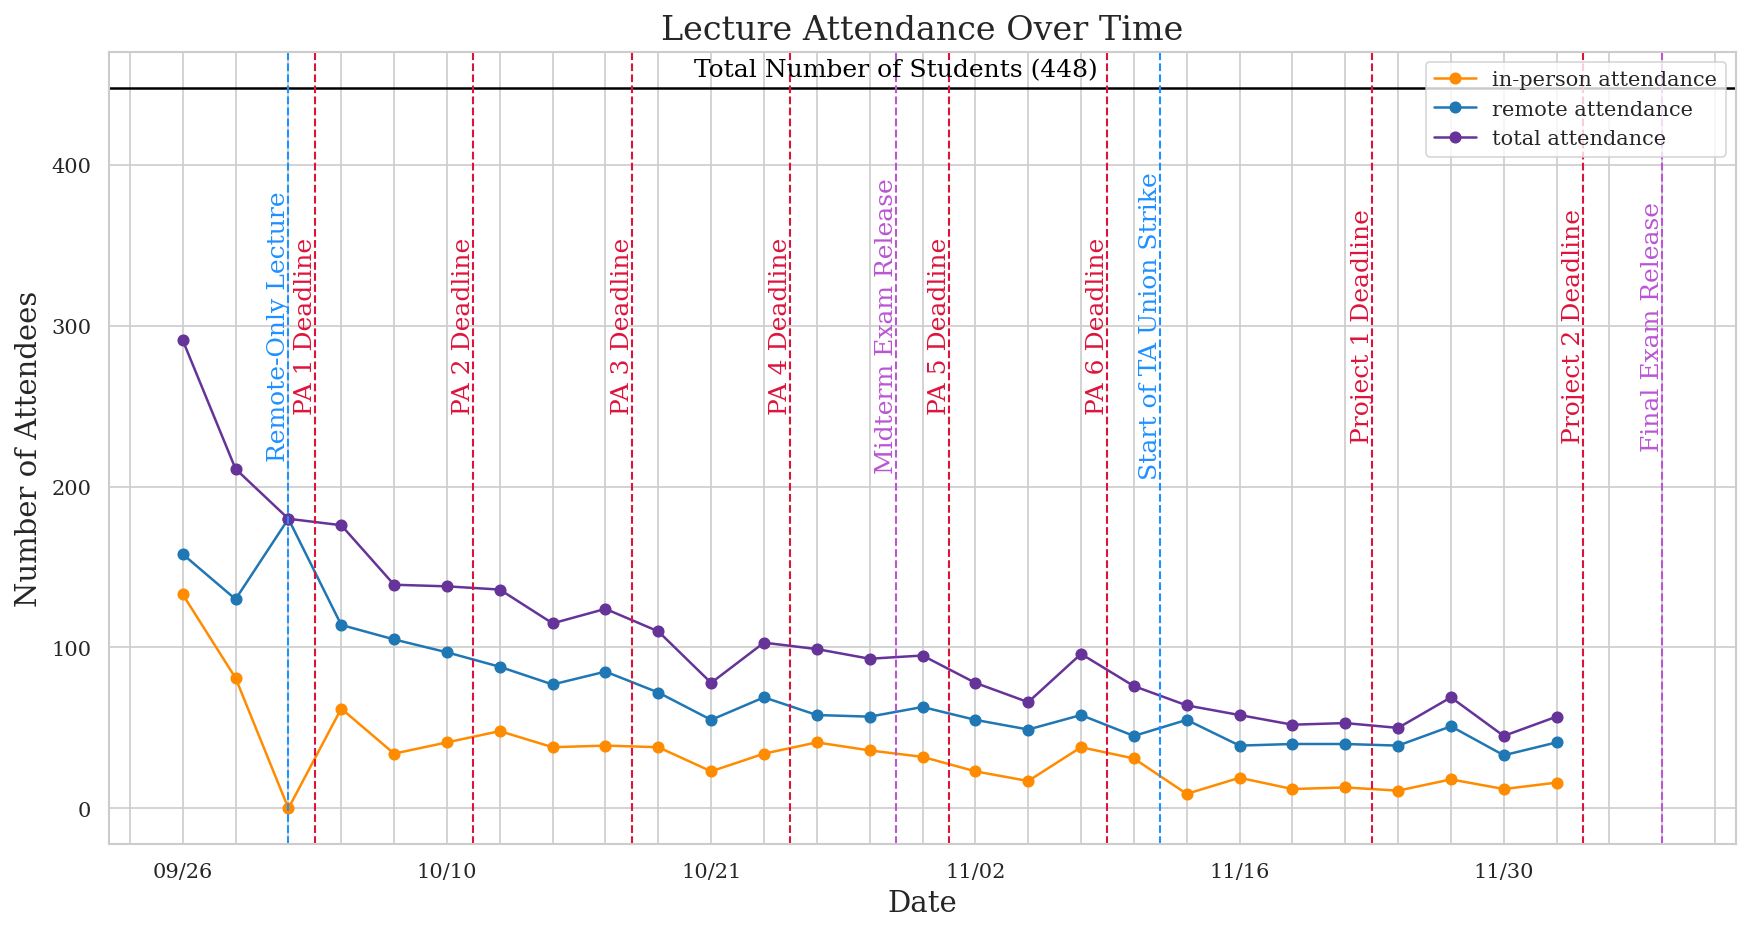
\includegraphics[width= 16cm]{figures/attendance_over_time.png}
    \caption{Synchronous attendance counts for the course lectures over time}
    \label{fig:attendance_over_time}
\end{figure}

As can be seen in Figure \ref{fig:attendance_over_time}, both in-person attendance and remote attendance gradually decreased over time, with certain events like the remote-only lecture and the start of the TA union strike having a noticeable correlation with each mode of attendance. In fact, those two events were the only points in the course other than the lecture after the midterm exam when the number of in-person attendees decreased and the number of remote attendees increased on the same day.

\section{Survey Results}

\subsection{Pre-Course Survey}

A total of 287 students submitted responses to the pre-course survey. For certain sections, the survey branched into separate questions for those it classified as hybrid/in-person attendees and those it classified as remote/asynchronous/non-attendees. Due to the low number of students who identified as a race that was not Asian or White, they were collectively classified as Other for the purposes of stratification. In addition, only a single student identified as a gender that was not male or female, so we limited our stratification based on gender to male and female students.

\begin{figure}[H]
    \vspace{5mm}
    \centering
    \textbf{In which section of the course are you officially enrolled? (N = 287)}\par\medskip
    \vspace{2mm}
    \begin{subfigure}[t]{1\textwidth}
        \centering
        \begin{tikzpicture}
            \begin{axis}[
                name=ax1,
                width=.4*\textwidth,
                height=9cm,
                major x tick style=transparent,
                ybar=2*\pgflinewidth,
                bar width=8pt,
                ymajorgrids=true,
                ylabel={Number of Responses},
                ylabel shift=-1mm,
                symbolic x coords={in-person,remote},
                xtick=data,
                x tick label style={
                    text width=6em,align=center,font=\small\linespread{0.8}\selectfont
                },
                scaled y ticks=false,
                enlarge x limits=.5,
                ymin=0,
                legend cell align=left,
                legend style={
                    at={(1.2,1.05)},
                    anchor=south,
                    column sep=1ex,
                    font=\footnotesize\linespread{.8}\selectfont,
                    /tikz/nodes={text width=4.5em,text height=.75em,text depth=,anchor=base},
                    align=left,
                    legend columns=5
                }
            ]
                \addplot[style={stand_1,fill=stand_1,mark=none}]
                    coordinates {(in-person,41) (remote,43)};
    
                \addplot[style={stand_2,fill=stand_2,mark=none}]
                    coordinates {(in-person,41) (remote,61)};
    
                \addplot[style={stand_3,fill=stand_3,mark=none}]
                    coordinates {(in-person,36) (remote,40)};
    
                \addplot[style={stand_4,fill=stand_4,mark=none}]
                    coordinates {(in-person,7) (remote,5)};
    
                \addplot[style={stand_5,fill=stand_5,mark=none}]
                    coordinates {(in-person,4) (remote,9)};

                \legend{2nd year,3rd year,4th year,5th+ year,Masters/PhD}
            \end{axis}at={(ax1.south east)},
            
            \begin{axis}[
                at={(ax1.south east)},
                xshift=2.5cm,
                width=.4*\textwidth,
                height=9cm,
                major x tick style=transparent,
                ybar=2*\pgflinewidth,
                bar width=8pt,
                ymajorgrids=true,
                ylabel={Percentage of Category},
                ylabel shift=-2mm,
                yticklabel={$\pgfmathprintnumber{\tick}\%$},
                ymin=0, ymax=100,
                extra y ticks={10,30,50,70,90},
                symbolic x coords={in-person,remote},
                xtick=data,
                x tick label style={
                    text width=6em,align=center,font=\small\linespread{0.8}\selectfont
                },
                scaled y ticks=false,
                enlarge x limits=.5,
                ymin=0,
            ]
                \addplot[style={stand_1,fill=stand_1,mark=none}]
                    coordinates {(in-person,48.81) (remote,51.19)};
    
                \addplot[style={stand_2,fill=stand_2,mark=none}]
                    coordinates {(in-person,40.20) (remote,59.80)};
    
                \addplot[style={stand_3,fill=stand_3,mark=none}]
                    coordinates {(in-person,47.37) (remote,52.63)};
    
                \addplot[style={stand_4,fill=stand_4,mark=none}]
                    coordinates {(in-person,58.33) (remote,41.67)};
    
                \addplot[style={stand_5,fill=stand_5,mark=none}]
                    coordinates {(in-person,30.77) (remote,69.23)};
            \end{axis}
        \end{tikzpicture}
        \caption{Stratified by class standing}
    \end{subfigure}
    \captionsetup{justification=centering}
    \caption{Number of respondents enrolled in each course section}
    \label{fig:enrollment_section}
\end{figure}

\begin{figure}[H]\ContinuedFloat
    \begin{subfigure}[t]{1\textwidth}
        \centering
        \begin{tikzpicture}
            \begin{axis}[
                name=ax1,
                width=.4*\textwidth,
                height=9cm,
                major x tick style=transparent,
                ybar=2*\pgflinewidth,
                bar width=8pt,
                ymajorgrids=true,
                ylabel={Number of Responses},
                ylabel shift=-1mm,
                symbolic x coords={in-person,remote},
                xtick=data,
                scaled y ticks=false,
                enlarge x limits=.5,
                ymin=0,
                legend cell align=left,
                legend style={
                    at={(1.2,1.05)},
                    anchor=south,
                    column sep=1ex,
                    font=\footnotesize\linespread{.8}\selectfont,
                    /tikz/nodes={text width=3em,text height=.75em,text depth=,anchor=base},
                    align=left,
                    legend columns=3
                }
            ]
                \addplot[style={race_1,fill=race_1,mark=none}]
                    coordinates {(in-person,21) (remote,29)};
    
                \addplot[style={race_2,fill=race_2,mark=none}]
                    coordinates {(in-person,100) (remote,128)};

                \addplot[style={race_3,fill=race_3,mark=none}]
                    coordinates {(in-person,8) (remote,12)};
                        
                \legend{White,Asian,Other}
            \end{axis}at={(ax1.south east)},
            
            \begin{axis}[
                at={(ax1.south east)},
                xshift=2.5cm,
                width=.4*\textwidth,
                height=9cm,
                major x tick style=transparent,
                ybar=2*\pgflinewidth,
                bar width=8pt,
                ymajorgrids=true,
                ylabel={Percentage of Category},
                ylabel shift=-2mm,
                yticklabel={$\pgfmathprintnumber{\tick}\%$},
                ymin=0, ymax=100,
                extra y ticks={10,30,50,70,90},
                symbolic x coords={in-person,remote},
                xtick=data,
                scaled y ticks=false,
                enlarge x limits=.5,
                ymin=0,
            ]
                \addplot[style={race_1,fill=race_1,mark=none}]
                    coordinates {(in-person,42.00) (remote,58.00)};
    
                \addplot[style={race_2,fill=race_2,mark=none}]
                    coordinates {(in-person,43.86) (remote,56.14)};
    
                \addplot[style={race_3,fill=race_3,mark=none}]
                    coordinates {(in-person,40.00) (remote,60.00)};
            \end{axis}
        \end{tikzpicture}
        \caption{Stratified by race}
    \end{subfigure}
    
    \begin{subfigure}[t]{1\textwidth}
        \vspace{5mm}
        \centering
        \begin{tikzpicture}
            \begin{axis}[
                name=ax1,
                width=.4*\textwidth,
                height=9cm,
                major x tick style=transparent,
                ybar=2*\pgflinewidth,
                bar width=8pt,
                ymajorgrids=true,
                ylabel={Number of Responses},
                ylabel shift=-1mm,
                symbolic x coords={in-person,remote},
                xtick=data,
                scaled y ticks=false,
                enlarge x limits=.5,
                ymin=0,
                legend cell align=left,
                legend style={
                    at={(1.2,1.05)},
                    anchor=south,
                    column sep=1ex,
                    font=\footnotesize\linespread{.8}\selectfont,
                    /tikz/nodes={text width=3em,text height=.75em,text depth=,anchor=base},
                    align=left,
                    legend columns=2
                }
            ]
                \addplot[style={gender_1,fill=gender_1,mark=none}]
                    coordinates {(in-person,86) (remote,124)};
    
                \addplot[style={gender_2,fill=gender_2,mark=none}]
                    coordinates {(in-person,40) (remote,31)};
        
                \legend{Male,Female}
            \end{axis}at={(ax1.south east)},
            
            \begin{axis}[
                at={(ax1.south east)},
                xshift=2.5cm,
                width=.4*\textwidth,
                height=9cm,
                major x tick style=transparent,
                ybar=2*\pgflinewidth,
                bar width=8pt,
                ymajorgrids=true,
                ylabel={Percentage of Category},
                ylabel shift=-2mm,
                yticklabel={$\pgfmathprintnumber{\tick}\%$},
                ymin=0, ymax=100,
                extra y ticks={10,30,50,70,90},
                symbolic x coords={in-person,remote},
                xtick=data,
                scaled y ticks=false,
                enlarge x limits=.5,
                ymin=0,
            ]
                \addplot[style={gender_1,fill=gender_1,mark=none}]
                    coordinates {(in-person,40.95) (remote,59.05)};
    
                \addplot[style={gender_2,fill=gender_2,mark=none}]
                    coordinates {(in-person,56.34) (remote,43.66)};
            \end{axis}
        \end{tikzpicture}
        \caption{Stratified by gender}
    \end{subfigure}
    \captionsetup{justification=centering}
    \caption[]{Number of respondents enrolled in each course section (cont.)}
\end{figure}

Students were asked to state which section they were enrolled in at the start of the course. Given that there were 189 students enrolled in the in-person section and 203 students enrolled in the remote section overall, 44.95\% of respondents were in-person enrollees, while 55.05\% were remote enrollees. In the days leading up to the enrollment deadline, we found that some students remained on the waitlist for the in-person section even while there were seats available in the remote section, despite the fact that they were identical in all but name.

When we stratify course enrollment by class standing, we see that third-year students made up a higher percentage of the enrollment for the remote section than the in-person section, at 38.6\% and 31.8\%. Other than this, however, enrollment was fairly even across the two sections. Neither race nor gender appeared to have a significant impact on a student's section of enrollment.

\begin{figure}[H]
    \vspace{5mm}
    \centering
    \textbf{Why did you choose to enroll in the in-person section? (N = 129)}\par\medskip
    \vspace{2mm}
    \begin{subfigure}[t]{1\textwidth}
        \centering
        \begin{tikzpicture}
            \begin{axis}[
                width=.85*\textwidth,
                height=9cm,
                major x tick style=transparent,
                ybar=2*\pgflinewidth,
                bar width=8pt,
                ymajorgrids=true,
                ylabel={Number of Responses},
                symbolic x coords={prefer in-person,easier to learn in-person,will already be on campus,will be unable to focus if remote},
                xtick=data,
                x tick label style={
                    text width=6em,align=center,font=\footnotesize\linespread{0.8}\selectfont
                },
                scaled y ticks=false,
                enlarge x limits=.25,
                ymin=0,
                legend cell align=left,
                legend style={
                    at={(.5,1.05)},
                    anchor=south,
                    column sep=1ex,
                    font=\footnotesize\linespread{.8}\selectfont,
                    /tikz/nodes={text width=4.5em,text height=.75em,text depth=,anchor=base},
                    align=left,
                    legend columns=5
                }
            ]
                \addplot[style={stand_1,fill=stand_1,mark=none}]
                coordinates {(prefer in-person,28) (easier to learn in-person,18) (will already be on campus,26) (will be unable to focus if remote,25)};

                \addplot[style={stand_2,fill=stand_2,mark=none}]
                    coordinates {(prefer in-person,19) (easier to learn in-person,18) (will already be on campus,15) (will be unable to focus if remote,21)};
    
                \addplot[style={stand_3,fill=stand_3,mark=none}]
                    coordinates {(prefer in-person,23) (easier to learn in-person,19) (will already be on campus,20) (will be unable to focus if remote,17)};
    
                \addplot[style={stand_4,fill=stand_4,mark=none}]
                    coordinates {(prefer in-person,4) (easier to learn in-person,4) (will already be on campus,1) (will be unable to focus if remote,5)};
    
                \addplot[style={stand_5,fill=stand_5,mark=none}]
                    coordinates {(prefer in-person,2) (easier to learn in-person,0) (will already be on campus,0) (will be unable to focus if remote,1)};
        
                \legend{2nd year,3rd year,4th year,5th+ year,Masters/PhD}
            \end{axis}
        
            \begin{axis}[
                yshift=-9cm,
                width=.85*\textwidth,
                height=9cm,
                major x tick style=transparent,
                ybar=2*\pgflinewidth,
                bar width=8pt,
                ymajorgrids=true,
                ylabel={Percentage of Category},
                ylabel shift=-2mm,
                yticklabel={$\pgfmathprintnumber{\tick}\%$},
                ymin=0, ymax=100,
                extra y ticks={10,30,50,70,90},
                symbolic x coords={prefer in-person,easier to learn in-person,will already be on campus,will be unable to focus if remote},
                xtick=data,
                x tick label style={
                    text width=6em,align=center,font=\footnotesize\linespread{0.8}\selectfont
                },
                scaled y ticks=false,
                enlarge x limits=.25,
                ymin=0,
            ]            
                \addplot[style={stand_1,fill=stand_1,mark=none}]
                coordinates {(prefer in-person,68.29) (easier to learn in-person,43.90) (will already be on campus,63.41) (will be unable to focus if remote,60.98)};

                \addplot[style={stand_2,fill=stand_2,mark=none}]
                    coordinates {(prefer in-person,46.34) (easier to learn in-person,43.90) (will already be on campus,36.59) (will be unable to focus if remote,51.22)};
    
                \addplot[style={stand_3,fill=stand_3,mark=none}]
                    coordinates {(prefer in-person,63.89) (easier to learn in-person,52.78) (will already be on campus,55.56) (will be unable to focus if remote,47.22)};
    
                \addplot[style={stand_4,fill=stand_4,mark=none}]
                    coordinates {(prefer in-person,57.14) (easier to learn in-person,57.14) (will already be on campus,14.29) (will be unable to focus if remote,71.43)};
    
                \addplot[style={stand_5,fill=stand_5,mark=none}]
                    coordinates {(prefer in-person,50.00) (easier to learn in-person,0.00) (will already be on campus,0.00) (will be unable to focus if remote,25.00)};
            \end{axis}
        \end{tikzpicture}
        \caption{Stratified by class standing}
    \end{subfigure}
    \captionsetup{justification=centering}
    \caption{Reasons why respondents enrolled in the in-person section}
    \label{fig:inperson_enrollment_reasons}
\end{figure}

\begin{figure}[H]\ContinuedFloat
    \centering
    \begin{subfigure}[t]{1\textwidth}
        \vspace{5mm}
        \centering
        \begin{tikzpicture}
            \begin{axis}[
                width=.9*\textwidth,
                height=9cm,
                major x tick style=transparent,
                ybar=2*\pgflinewidth,
                bar width=8pt,
                ymajorgrids=true,
                ylabel={Number of Responses},
                symbolic x coords={prefer in-person,easier to learn in-person,will already be on campus,will be unable to focus if remote},
                xtick=data,
                x tick label style={
                    text width=6em,align=center,font=\footnotesize\linespread{0.8}\selectfont
                },
                scaled y ticks=false,
                enlarge x limits=.15,
                ymin=0,
                legend cell align=left,
                legend style={
                    at={(.5,1.05)},
                    anchor=south,
                    column sep=1ex,
                    font=\footnotesize\linespread{.8}\selectfont,
                    /tikz/nodes={text width=3em,text height=.75em,text depth=,anchor=base},
                    align=left,
                    legend columns=3
                }
            ]
                \addplot[style={race_1,fill=race_1,mark=none}]
                coordinates {(prefer in-person,15) (easier to learn in-person,12) (will already be on campus,12) (will be unable to focus if remote,11)};
    
                \addplot[style={race_2,fill=race_2,mark=none}]
                coordinates {(prefer in-person,54) (easier to learn in-person,43) (will already be on campus,46) (will be unable to focus if remote,53)};
    
                \addplot[style={race_3,fill=race_3,mark=none}]
                coordinates {(prefer in-person,6) (easier to learn in-person,3) (will already be on campus,5) (will be unable to focus if remote,4)};
        
                \legend{White,Asian,Other}
            \end{axis}
        
            \begin{axis}[
                yshift=-9cm,
                width=.9*\textwidth,
                height=9cm,
                major x tick style=transparent,
                ybar=2*\pgflinewidth,
                bar width=8pt,
                ymajorgrids=true,
                ylabel={Percentage of Category},
                ylabel shift=-2mm,
                yticklabel={$\pgfmathprintnumber{\tick}\%$},
                ymin=0, ymax=100,
                extra y ticks={10,30,50,70,90},
                symbolic x coords={prefer in-person,easier to learn in-person,will already be on campus,will be unable to focus if remote},
                xtick=data,
                x tick label style={
                    text width=6em,align=center,font=\footnotesize\linespread{0.8}\selectfont
                },
                scaled y ticks=false,
                enlarge x limits=.15,
                ymin=0,
            ]
                \addplot[style={race_1,fill=race_1,mark=none}]
                coordinates {(prefer in-person,71.43) (easier to learn in-person,57.14) (will already be on campus,57.14) (will be unable to focus if remote,52.38)};
    
                \addplot[style={race_2,fill=race_2,mark=none}]
                coordinates {(prefer in-person,54.00) (easier to learn in-person,43.00) (will already be on campus,46.00) (will be unable to focus if remote,53.00)};
    
                \addplot[style={race_3,fill=race_3,mark=none}]
                coordinates {(prefer in-person,75.00) (easier to learn in-person,37.5) (will already be on campus,62.5) (will be unable to focus if remote,50.00)};
            \end{axis}
        \end{tikzpicture}
        \caption{Stratified by race}
    \end{subfigure}
    \captionsetup{justification=centering}
    \caption[]{Reasons why respondents enrolled in the in-person section (cont.)}
\end{figure}

\begin{figure}[H]\ContinuedFloat
    \centering
    \begin{subfigure}[t]{1\textwidth}
        \centering
        \begin{tikzpicture}
            \begin{axis}[
                width=.9*\textwidth,
                height=9cm,
                major x tick style=transparent,
                ybar=2*\pgflinewidth,
                bar width=8pt,
                ymajorgrids=true,
                ylabel={Number of Responses},
                symbolic x coords={prefer in-person,easier to learn in-person,will already be on campus,will be unable to focus if remote},
                xtick=data,
                x tick label style={
                    text width=6em,align=center,font=\footnotesize\linespread{0.8}\selectfont
                },
                scaled y ticks=false,
                enlarge x limits=.15,
                ymin=0,
                legend cell align=left,
                legend style={
                    at={(.5,1.05)},
                    anchor=south,
                    column sep=1ex,
                    font=\footnotesize\linespread{.8}\selectfont,
                    /tikz/nodes={text width=3em,text height=.75em,text depth=,anchor=base},
                    align=left,
                    legend columns=2
                }
            ]
                \addplot[style={gender_1,fill=gender_1,mark=none}]
                coordinates {(prefer in-person,52) (easier to learn in-person,39) (will already be on campus,42) (will be unable to focus if remote,44)};
    
                \addplot[style={gender_2,fill=gender_2,mark=none}]
                coordinates {(prefer in-person,21) (easier to learn in-person,19) (will already be on campus,19) (will be unable to focus if remote,23)};
        
                \legend{Male,Female}
            \end{axis},
            
            \begin{axis}[
                yshift=-9cm,
                width=.9*\textwidth,
                height=9cm,
                major x tick style=transparent,
                ybar=2*\pgflinewidth,
                bar width=8pt,
                ymajorgrids=true,
                ylabel={Percentage of Category},
                ylabel shift=-2mm,
                yticklabel={$\pgfmathprintnumber{\tick}\%$},
                ymin=0, ymax=100,
                extra y ticks={10,30,50,70,90},
                symbolic x coords={prefer in-person,easier to learn in-person,will already be on campus,will be unable to focus if remote},
                xtick=data,
                x tick label style={
                    text width=6em,align=center,font=\footnotesize\linespread{0.8}\selectfont
                },
                scaled y ticks=false,
                enlarge x limits=.15,
                ymin=0,
            ]
                \addplot[style={gender_1,fill=gender_1,mark=none}]
                coordinates {(prefer in-person,60.47) (easier to learn in-person,45.35) (will already be on campus,48.84) (will be unable to focus if remote,51.16)};
    
                \addplot[style={gender_2,fill=gender_2,mark=none}]
                coordinates {(prefer in-person,52.5) (easier to learn in-person,47.5) (will already be on campus,47.5) (will be unable to focus if remote,57.5)};
            \end{axis}
        \end{tikzpicture}
        \caption{Stratified by gender}
    \end{subfigure}
    \captionsetup{justification=centering}
    \caption[]{Reasons why respondents enrolled in the in-person section (cont.)}
    \vspace{10mm}
\end{figure}

129 of the pre-course survey respondents were enrolled in the in-person section. When asked why they did so, 58.9\% stated that they preferred to learn in an in-person environment, 45.7\% stated that they found it easier to learn in person, 48.1\% stated that they would already be on campus when lectures took place, and 53.5\% expressed concern that they would be unable to focus if they attended remotely (see Figure \ref{fig:inperson_enrollment_reasons}). Though only about half of the respondents selected each of the available reasons, the fact that at least one of these reasons was selected by every respondent enrolled in the in-person section shows that they did so out of some level of preference for in-person instruction over remote instruction.

When we stratify by class standing, we see that the second-year students were most likely to find the in-person section convenient due to already being on campus. We expected this to be the case, since on-campus housing is only guaranteed for undergraduate students up to the end of their second year of enrollment. Other than this, however, the reasons were fairly proportional with class standing. In addition, reasons were even across students of different races and genders.

% When in-person enrollees were asked how often they planned to attend lectures in person, 69.0\% said they would attend as often as possible (i.e., three times a week). This indicates that, while actual in-person attendance was much lower, a majority of students in the in-person section had intended to engage with the in-person modality of the course when they started.

\begin{figure}[H]
    \vspace{5mm}
    \centering
    \textbf{Why did you choose to enroll in the remote section? (N = 158)}\par\medskip
    \vspace{2mm}
    \begin{subfigure}[t]{1\textwidth}
        \centering
        \begin{tikzpicture}
            \begin{axis}[
                width=.85*\textwidth,
                height=9cm,
                major x tick style=transparent,
                ybar=2*\pgflinewidth,
                bar width=8pt,
                ymajorgrids=true,
                ylabel={Number of Responses},
                symbolic x coords={prefer remote,easier to learn remote,unable to get to campus,concerned for health,in-person section was full},
                xtick=data,
                x tick label style={
                    text width=6em,align=center,font=\footnotesize\linespread{0.8}\selectfont
                },
                scaled y ticks=false,
                enlarge x limits=.25,
                ymin=0,
                legend cell align=left,
                legend style={
                    at={(.5,1.05)},
                    anchor=south,
                    column sep=1ex,
                    font=\footnotesize\linespread{.8}\selectfont,
                    /tikz/nodes={text width=4.5em,text height=.75em,text depth=,anchor=base},
                    align=left,
                    legend columns=5
                }
            ]
                \addplot[style={stand_1,fill=stand_1,mark=none}]
                    coordinates {(prefer remote,15) (easier to learn remote,7) (unable to get to campus,3) (concerned for health,2) (in-person section was full,31)};
    
                \addplot[style={stand_2,fill=stand_2,mark=none}]
                    coordinates {(prefer remote,21) (easier to learn remote,20) (unable to get to campus,13) (concerned for health,7) (in-person section was full,36)};
    
                \addplot[style={stand_3,fill=stand_3,mark=none}]
                    coordinates {(prefer remote,19) (easier to learn remote,14) (unable to get to campus,12) (concerned for health,6) (in-person section was full,21)};
    
                \addplot[style={stand_4,fill=stand_4,mark=none}]
                    coordinates {(prefer remote,2) (easier to learn remote,1) (unable to get to campus,3) (concerned for health,0) (in-person section was full,2)};
    
                \addplot[style={stand_5,fill=stand_5,mark=none}]
                    coordinates {(prefer remote,5) (easier to learn remote,2) (unable to get to campus,1) (concerned for health,0) (in-person section was full,7)};
        
                \legend{2nd year,3rd year,4th year,5th+ year,Masters/PhD}
            \end{axis}
        
            \begin{axis}[
                yshift=-9cm,
                width=.85*\textwidth,
                height=9cm,
                major x tick style=transparent,
                ybar=2*\pgflinewidth,
                bar width=8pt,
                ymajorgrids=true,
                ylabel={Percentage of Category},
                ylabel shift=-2mm,
                yticklabel={$\pgfmathprintnumber{\tick}\%$},
                ymin=0, ymax=100,
                extra y ticks={10,30,50,70,90},
                symbolic x coords={prefer remote,easier to learn remote,unable to get to campus,concerned for health,in-person section was full},
                xtick=data,
                x tick label style={
                    text width=6em,align=center,font=\footnotesize\linespread{0.8}\selectfont
                },
                scaled y ticks=false,
                enlarge x limits=.25,
                ymin=0,
            ]            
                \addplot[style={stand_1,fill=stand_1,mark=none}]
                    coordinates {(prefer remote,34.88) (easier to learn remote,16.28) (unable to get to campus,6.98) (concerned for health,4.65) (in-person section was full,72.09)};
    
                \addplot[style={stand_2,fill=stand_2,mark=none}]
                    coordinates {(prefer remote,34.43) (easier to learn remote,32.79) (unable to get to campus,21.31) (concerned for health,11.48) (in-person section was full,59.02)};
    
                \addplot[style={stand_3,fill=stand_3,mark=none}]
                    coordinates {(prefer remote,47.50) (easier to learn remote,35.00) (unable to get to campus,30.00) (concerned for health,15.00) (in-person section was full,52.50)};
    
                \addplot[style={stand_4,fill=stand_4,mark=none}]
                    coordinates {(prefer remote,40.00) (easier to learn remote,20.00) (unable to get to campus,60.00) (concerned for health,0.00) (in-person section was full,40.00)};
    
                \addplot[style={stand_5,fill=stand_5,mark=none}]
                    coordinates {(prefer remote,55.56) (easier to learn remote,22.22) (unable to get to campus,11.11) (concerned for health,0.00) (in-person section was full,77.78)};
            \end{axis}
        \end{tikzpicture}
        \caption{Stratified by class standing}
    \end{subfigure}
    \captionsetup{justification=centering}
    \caption{Reasons why respondents enrolled in the remote section}
    \label{fig:remote_enrollment_reasons}
\end{figure}

\begin{figure}[H]\ContinuedFloat
    \centering
    \begin{subfigure}[t]{1\textwidth}
        \vspace{5mm}
        \centering
        \begin{tikzpicture}
            \begin{axis}[
                width=.9*\textwidth,
                height=9cm,
                major x tick style=transparent,
                ybar=2*\pgflinewidth,
                bar width=8pt,
                ymajorgrids=true,
                ylabel={Number of Responses},
                symbolic x coords={prefer remote,easier to learn remote,unable to get to campus,concerned for health,in-person section was full},
                xtick=data,
                x tick label style={
                    text width=6em,align=center,font=\footnotesize\linespread{0.8}\selectfont
                },
                scaled y ticks=false,
                enlarge x limits=.15,
                ymin=0,
                legend cell align=left,
                legend style={
                    at={(.5,1.05)},
                    anchor=south,
                    column sep=1ex,
                    font=\footnotesize\linespread{.8}\selectfont,
                    /tikz/nodes={text width=3em,text height=.75em,text depth=,anchor=base},
                    align=left,
                    legend columns=3
                }
            ]
                \addplot[style={race_1,fill=race_1,mark=none}]
                    coordinates {(prefer remote,11) (easier to learn remote,6) (unable to get to campus,5) (concerned for health,1) (in-person section was full,20)};
        
                \addplot[style={race_2,fill=race_2,mark=none}]
                    coordinates {(prefer remote,52) (easier to learn remote,38) (unable to get to campus,26) (concerned for health,14) (in-person section was full,78)};
    
                \addplot[style={race_3,fill=race_3,mark=none}]
                    coordinates {(prefer remote,3) (easier to learn remote,2) (unable to get to campus,3) (concerned for health,0) (in-person section was full,6)};
    
                \legend{White,Asian,Other}
            \end{axis}
        
            \begin{axis}[
                yshift=-9cm,
                width=.9*\textwidth,
                height=9cm,
                major x tick style=transparent,
                ybar=2*\pgflinewidth,
                bar width=8pt,
                ymajorgrids=true,
                ylabel={Percentage of Category},
                ylabel shift=-2mm,
                yticklabel={$\pgfmathprintnumber{\tick}\%$},
                ymin=0, ymax=100,
                extra y ticks={10,30,50,70,90},
                symbolic x coords={prefer remote,easier to learn remote,unable to get to campus,concerned for health,in-person section was full},
                xtick=data,
                x tick label style={
                    text width=6em,align=center,font=\footnotesize\linespread{0.8}\selectfont
                },
                scaled y ticks=false,
                enlarge x limits=.15,
                ymin=0,
            ]
                \addplot[style={race_1,fill=race_1,mark=none}]
                    coordinates {(prefer remote,37.93) (easier to learn remote,20.69) (unable to get to campus,17.24) (concerned for health,3.45) (in-person section was full,68.97)};
        
                \addplot[style={race_2,fill=race_2,mark=none}]
                    coordinates {(prefer remote,40.63) (easier to learn remote,29.69) (unable to get to campus,20.31) (concerned for health,10.94) (in-person section was full,60.94)};
    
                \addplot[style={race_3,fill=race_3,mark=none}]
                    coordinates {(prefer remote,33.33) (easier to learn remote,22.22) (unable to get to campus,33.33) (concerned for health,0.00) (in-person section was full,66.67)};
            \end{axis}
        \end{tikzpicture}
        \caption{Stratified by race}
    \end{subfigure}
    \captionsetup{justification=centering}
    \caption[]{Reasons why respondents enrolled in the remote section (cont.)}
\end{figure}

\begin{figure}[H]\ContinuedFloat
    \centering
    \begin{subfigure}[t]{1\textwidth}
        \centering
        \begin{tikzpicture}
            \begin{axis}[
                width=.9*\textwidth,
                height=9cm,
                major x tick style=transparent,
                ybar=2*\pgflinewidth,
                bar width=8pt,
                ymajorgrids=true,
                ylabel={Number of Responses},
                symbolic x coords={prefer remote,easier to learn remote,unable to get to campus,concerned for health,in-person section was full},
                xtick=data,
                x tick label style={
                    text width=6em,align=center,font=\footnotesize\linespread{0.8}\selectfont
                },
                scaled y ticks=false,
                enlarge x limits=.15,
                ymin=0,
                legend cell align=left,
                legend style={
                    at={(.5,1.05)},
                    anchor=south,
                    column sep=1ex,
                    font=\footnotesize\linespread{.8}\selectfont,
                    /tikz/nodes={text width=3em,text height=.75em,text depth=,anchor=base},
                    align=left,
                    legend columns=2
                }
            ]
                \addplot[style={gender_1,fill=gender_1,mark=none}]
                    coordinates {(prefer remote,55) (easier to learn remote,39) (unable to get to campus,24) (concerned for health,14) (in-person section was full,75)};
    
                \addplot[style={gender_2,fill=gender_2,mark=none}]
                    coordinates {(prefer remote,6) (easier to learn remote,4) (unable to get to campus,7) (concerned for health,0) (in-person section was full,20)};
        
                \legend{Male,Female}
            \end{axis},
            
            \begin{axis}[
                yshift=-9cm,
                width=.9*\textwidth,
                height=9cm,
                major x tick style=transparent,
                ybar=2*\pgflinewidth,
                bar width=8pt,
                ymajorgrids=true,
                ylabel={Percentage of Category},
                ylabel shift=-2mm,
                yticklabel={$\pgfmathprintnumber{\tick}\%$},
                ymin=0, ymax=100,
                extra y ticks={10,30,50,70,90},
                symbolic x coords={prefer remote,easier to learn remote,unable to get to campus,concerned for health,in-person section was full},
                xtick=data,
                x tick label style={
                    text width=6em,align=center,font=\footnotesize\linespread{0.8}\selectfont
                },
                scaled y ticks=false,
                enlarge x limits=.15,
                ymin=0,
            ]
                \addplot[style={gender_1,fill=gender_1,mark=none}]
                    coordinates {(prefer remote,44.35) (easier to learn remote,31.45) (unable to get to campus,19.35) (concerned for health,11.29) (in-person section was full,60.48)};
    
                \addplot[style={gender_2,fill=gender_2,mark=none}]
                    coordinates {(prefer remote,19.35) (easier to learn remote,12.90) (unable to get to campus,22.58) (concerned for health,0.00) (in-person section was full,64.52)};
            \end{axis}
        \end{tikzpicture}
        \caption{Stratified by gender}
    \end{subfigure}
    \captionsetup{justification=centering}
    \caption[]{Reasons why respondents enrolled in the remote section (cont.)}
    \vspace{10mm}
\end{figure}

158 of the pre-course survey respondents were enrolled in the remote section. When asked why they did so, 39.2\% stated that they preferred to learn in a remote environment, 27.8\% stated that they found it easier to learn remotely, 20.3\% stated that they would be unable to get to campus for the lectures, and 61.4\% stated that they did so simply because the in-person section was full (see Figure \ref{fig:remote_enrollment_reasons}). By a large margin, the most common reason that students had enrolled in the remote section was because they were unable to enroll in the in-person section. This may have been due to the fact that the remote section was listed under a new course code and therefore made students unsure as to whether it would fulfill the same requirements as the in-person section.

When we stratify students' reasons for remote section enrollment by their class standing, we see further evidence that students were hesitant to enroll in the remote section due to the new course code: proportionally, second-year undergraduate students and graduate students were more likely than students of other class standings to indicate that they had done so because the in-person section was full. Students who were earlier on in their undergraduate degree may have been more cautious about whether their requirements would be met because this course is a prerequisite to many other upper-division courses in the department, making it a critical requirement for students in their second year. Meanwhile, graduate students may have also been more cautious about enrolling in the in-person section because they were unsure whether the remote section would fulfill their elective requirement. Stratifying by race does not reveal any significant differences in reasoning across students of different races; however, stratifying by gender reveals that male students are twice as likely to prefer remote courses and find it easy to learn in remote courses as female students.

% Remote enrollees were asked whether they planned to attend an in-person lecture at some point during the course: 47.5\% said that they did, 12.0\% said that they did not, and 40.5\% said that they were not yet sure. This matches the previous responses indicating that many students were only enrolled in the remote section because the in-person section was full.

\begin{figure}[H]
    \vspace{5mm}
    \centering
    \textbf{If this course was only offered as either an in-person or a remote course, which modality would you prefer? (N = 287)}\par\medskip
    \vspace{2mm}
    \begin{subfigure}[t]{1\textwidth}
        \centering
        \begin{tikzpicture}
            \begin{axis}[
                width=.7*\textwidth,
                height=9cm,
                major x tick style=transparent,
                ybar=2*\pgflinewidth,
                bar width=8pt,
                ymajorgrids=true,
                ylabel={Number of Responses},
                symbolic x coords={in-person,remote,neither},
                xtick=data,
                x tick label style={
                    text width=6em,align=center,font=\footnotesize\linespread{0.8}\selectfont
                },
                scaled y ticks=false,
                enlarge x limits=.25,
                ymin=0,
                legend cell align=left,
                legend style={
                    at={(.5,1.05)},
                    anchor=south,
                    column sep=1ex,
                    font=\footnotesize\linespread{.8}\selectfont,
                    /tikz/nodes={text width=4.5em,text height=.75em,text depth=,anchor=base},
                    align=left,
                    legend columns=5
                }
            ]
                \addplot[style={stand_1,fill=stand_1,mark=none}]
                    coordinates {(in-person,43) (remote,24) (neither,17)};

                \addplot[style={stand_2,fill=stand_2,mark=none}]
                    coordinates {(in-person,39) (remote,41) (neither,22)};
    
                \addplot[style={stand_3,fill=stand_3,mark=none}]
                    coordinates {(in-person,24) (remote,33) (neither,19)};
    
                \addplot[style={stand_4,fill=stand_4,mark=none}]
                    coordinates {(in-person,5) (remote,6) (neither,1)};
    
                \addplot[style={stand_5,fill=stand_5,mark=none}]
                    coordinates {(in-person,1) (remote,10) (neither,2)};
        
                \legend{2nd year,3rd year,4th year,5th+ year,Masters/PhD}
            \end{axis}
        
            \begin{axis}[
                yshift=-9cm,
                width=.7*\textwidth,
                height=9cm,
                major x tick style=transparent,
                ybar=2*\pgflinewidth,
                bar width=8pt,
                ymajorgrids=true,
                ylabel={Percentage of Category},
                ylabel shift=-2mm,
                yticklabel={$\pgfmathprintnumber{\tick}\%$},
                ymin=0, ymax=100,
                extra y ticks={10,30,50,70,90},
                symbolic x coords={in-person,remote,neither},
                xtick=data,
                x tick label style={
                    text width=6em,align=center,font=\footnotesize\linespread{0.8}\selectfont
                },
                scaled y ticks=false,
                enlarge x limits=.25,
                ymin=0,
            ]            
                \addplot[style={stand_1,fill=stand_1,mark=none}]
                    coordinates {(in-person,51.19) (remote,28.57) (neither,20.24)};

                \addplot[style={stand_2,fill=stand_2,mark=none}]
                    coordinates {(in-person,38.24) (remote,40.20) (neither,21.57)};
    
                \addplot[style={stand_3,fill=stand_3,mark=none}]
                    coordinates {(in-person,31.58) (remote,43.42) (neither,25.00)};
    
                \addplot[style={stand_4,fill=stand_4,mark=none}]
                    coordinates {(in-person,41.67) (remote,50.00) (neither,8.33)};
    
                \addplot[style={stand_5,fill=stand_5,mark=none}]
                    coordinates {(in-person,7.69) (remote,76.92) (neither,15.38)};
            \end{axis}
        \end{tikzpicture}
        \caption{Stratified by class standing}
    \end{subfigure}
    \captionsetup{justification=centering}
    \caption{Respondents who would have preferred either an in-person or a remote course}
    \label{fig:modality_preference}
\end{figure}

\begin{figure}[H]\ContinuedFloat
    \centering
    \begin{subfigure}[t]{1\textwidth}
        \vspace{5mm}
        \centering
        \begin{tikzpicture}
            \begin{axis}[
                width=.6*\textwidth,
                height=9cm,
                major x tick style=transparent,
                ybar=2*\pgflinewidth,
                bar width=8pt,
                ymajorgrids=true,
                ylabel={Number of Responses},
                symbolic x coords={in-person,remote,neither},
                xtick=data,
                x tick label style={
                    text width=6em,align=center,font=\footnotesize\linespread{0.8}\selectfont
                },
                scaled y ticks=false,
                enlarge x limits=.25,
                ymin=0,
                legend cell align=left,
                legend style={
                    at={(.5,1.05)},
                    anchor=south,
                    column sep=1ex,
                    font=\footnotesize\linespread{.8}\selectfont,
                    /tikz/nodes={text width=3em,text height=.75em,text depth=,anchor=base},
                    align=left,
                    legend columns=3
                }
            ]
                \addplot[style={race_1,fill=race_1,mark=none}]
                    coordinates {(in-person,28) (remote,13) (neither,9)};

                \addplot[style={race_2,fill=race_2,mark=none}]
                    coordinates {(in-person,80) (remote,98) (neither,50)};

                \addplot[style={race_3,fill=race_3,mark=none}]
                    coordinates {(in-person,6) (remote,8) (neither,3)};

                \legend{White,Asian,Other}
            \end{axis}
        
            \begin{axis}[
                yshift=-9cm,
                width=.6*\textwidth,
                height=9cm,
                major x tick style=transparent,
                ybar=2*\pgflinewidth,
                bar width=8pt,
                ymajorgrids=true,
                ylabel={Percentage of Category},
                ylabel shift=-2mm,
                yticklabel={$\pgfmathprintnumber{\tick}\%$},
                ymin=0, ymax=100,
                extra y ticks={10,30,50,70,90},
                symbolic x coords={in-person,remote,neither},
                xtick=data,
                x tick label style={
                    text width=6em,align=center,font=\footnotesize\linespread{0.8}\selectfont
                },
                scaled y ticks=false,
                enlarge x limits=.25,
                ymin=0,
            ]
                \addplot[style={race_1,fill=race_1,mark=none}]
                    coordinates {(in-person,56.00) (remote,26.00) (neither,18.00)};

                \addplot[style={race_2,fill=race_2,mark=none}]
                    coordinates {(in-person,35.09) (remote,42.98) (neither,21.93)};

                \addplot[style={race_3,fill=race_3,mark=none}]
                    coordinates {(in-person,35.29) (remote,47.06) (neither,17.65)};
            \end{axis}
        \end{tikzpicture}
        \caption{Stratified by race}
    \end{subfigure}
    \captionsetup{justification=centering}
    \caption[]{Respondents who would have preferred either an in-person or a remote course (cont.)}
\end{figure}

\begin{figure}[H]\ContinuedFloat
    \centering
    \begin{subfigure}[t]{1\textwidth}
        \centering
        \begin{tikzpicture}
            \begin{axis}[
                width=.6*\textwidth,
                height=9cm,
                major x tick style=transparent,
                ybar=2*\pgflinewidth,
                bar width=8pt,
                ymajorgrids=true,
                ylabel={Number of Responses},
                symbolic x coords={in-person,remote,neither},
                xtick=data,
                x tick label style={
                    text width=6em,align=center,font=\footnotesize\linespread{0.8}\selectfont
                },
                scaled y ticks=false,
                enlarge x limits=.25,
                ymin=0,
                legend cell align=left,
                legend style={
                    at={(.5,1.05)},
                    anchor=south,
                    column sep=1ex,
                    font=\footnotesize\linespread{.8}\selectfont,
                    /tikz/nodes={text width=3em,text height=.75em,text depth=,anchor=base},
                    align=left,
                    legend columns=2
                }
            ]
                \addplot[style={gender_1,fill=gender_1,mark=none}]
                    coordinates {(in-person,74) (remote,96) (neither,40)};
    
                \addplot[style={gender_2,fill=gender_2,mark=none}]
                    coordinates {(in-person,35) (remote,17) (neither,19)};
        
                \legend{Male,Female}
            \end{axis},
            
            \begin{axis}[
                yshift=-9cm,
                width=.6*\textwidth,
                height=9cm,
                major x tick style=transparent,
                ybar=2*\pgflinewidth,
                bar width=8pt,
                ymajorgrids=true,
                ylabel={Percentage of Category},
                ylabel shift=-2mm,
                yticklabel={$\pgfmathprintnumber{\tick}\%$},
                ymin=0, ymax=100,
                extra y ticks={10,30,50,70,90},
                symbolic x coords={in-person,remote,neither},
                xtick=data,
                x tick label style={
                    text width=6em,align=center,font=\footnotesize\linespread{0.8}\selectfont
                },
                scaled y ticks=false,
                enlarge x limits=.25,
                ymin=0,
            ]
                \addplot[style={gender_1,fill=gender_1,mark=none}]
                    coordinates {(in-person,35.24) (remote,45.71) (neither,19.05)};
    
                \addplot[style={gender_2,fill=gender_2,mark=none}]
                    coordinates {(in-person,49.30) (remote,23.94) (neither,26.76)};
            \end{axis}
        \end{tikzpicture}
        \caption{Stratified by gender}
    \end{subfigure}
    \captionsetup{justification=centering}
    \caption[]{Respondents who would have preferred either an in-person or a remote course (cont.)}
    \vspace{10mm}
\end{figure}

When all respondents were asked whether they would prefer to enroll in the course if it was only in-person or only remote, 39\% said that they would prefer in-person, 39.7\% said that they would prefer remote, and 21.3\% said that they did not have a preference either way. The fact that an almost identical number of students preferred in-person and remote modalities indicated that students looked for different things in their courses and had enrolled under different circumstances.

If we look at modality preference stratified by class standing, we see that second-year undergraduate students were more likely to prefer an in-person course, while graduate students were more likely to prefer a remote course. Interestingly, the differences in preferences were much greater than the actual proportions of students in different class standings that were enrolled in each section of the course (as seen in Figure \ref{fig:enrollment_section}), which is why we used this metric to stratify students' actual modality of attendance in Table \ref{tab:attendance-initial-preference}. When we stratify by race, we see that White students were most likely to prefer an in-person course; however, preferences were fairly uniform across students of different races apart from that. And when we stratify by gender, we see that female students were more likely to prefer an in-person course than male students, while male students were more likely to prefer a remote course than female students.

\subsection{Mid-Course and End-of-Course Surveys}

A total of 144 students submitted responses to the mid-course survey, while 232 students submitted responses to the end-of-course survey. Similarly to the pre-course survey, the mid-course and end-of-course surveys branched into separate questions for hybrid/in-person attendees and remote/asynchronous/non-attendees during the period of time preceding their distribution: the mid-course survey measured attendance for Weeks 1 to 5, while the end-of-course survey measured attendance for Weeks 6 to 10.

\begin{figure}[H]
    \vspace{5mm}
    \centering
    \textbf{Which of the following reasons have enabled you to keep attending lectures in person?}\par\medskip
    \vspace{2mm}
    \begin{subfigure}[t]{1\textwidth}
        \centering
        \hspace{-10mm}
        \begin{tikzpicture}[x={(.125,0)}, y={(0,.9)}]
            \tikzstyle{block} = [text width = 15em, align = right, font = \footnotesize\linespread{0.8}\selectfont];
            \foreach  \l/\x/\c[count=\y] in {{None of the above}/0/none,
                {I am already near the lecture hall on those days, so it is more convenient.}/7/attend_3,
                {I live on/near campus.}/17/attend_6,
                {I enjoy the level of engagement involved in attending lectures in person.}/18/attend_4,
                {I feel more involved in the class community when I attend lectures in person.}/19/attend_5,
                {It is easier for me to learn in an in-person setting.}/33/attend_2,
                {I prefer to learn in an in-person setting.}/34/attend_1}
            {
            \node[left, block] at (0,\y) {\l};
            \fill[\c] (0,\y-.4) rectangle (\x,\y+.4);
            \node[right] at (\x, \y) {\x};
            \node[right] at (\x+4, \y-.03) {($\pgfmathparse{\x / 41 * 100}\pgfmathprintnumber[precision=1]{\pgfmathresult}$\%)};}
            \draw (0,0) -- (55,0);
            \foreach \x in {10, 20, ..., 50}
            {\draw (\x,.2) -- (\x,0) node[below] {\x};}
            \draw (0,0) -- (0,7.5);
            \draw node[below] at (25,-0.6) {Number of Responses};
        \end{tikzpicture}
        \caption{Mid-course survey (N = 41)}
    \end{subfigure}
    
    \begin{subfigure}[t]{1\textwidth}
        \vspace{5mm}
        \centering
        \hspace{-10mm}
        \begin{tikzpicture}[x={(.125,0)}, y={(0,.9)}]
            \tikzstyle{block} = [text width = 15em, align = right, font = \footnotesize\linespread{0.8}\selectfont];
            \foreach  \l/\x/\c[count=\y] in {{None of the above}/2/none,
                {I am already near the lecture hall on those days, so it is more convenient.}/12/attend_3,
                {I live on/near campus.}/13/attend_6,
                {I feel more involved in the class community when I attend lectures in person.}/18/attend_5,
                {I enjoy the level of engagement involved in attending lectures in person.}/19/attend_4,
                {It is easier for me to learn in an in-person setting.}/25/attend_2,
                {I prefer to learn in an in-person setting.}/28/attend_1}
            {
            \node[left, block] at (0,\y) {\l};
            \fill[\c] (0,\y-.4) rectangle (\x,\y+.4);
            \node[right] at (\x, \y) {\x};
            \node[right] at (\x+4, \y-.03) {($\pgfmathparse{\x / 39 * 100}\pgfmathprintnumber[precision=1]{\pgfmathresult}$\%)};}
            \draw (0,0) -- (55,0);
            \foreach \x in {10, 20, ..., 50}
            {\draw (\x,.2) -- (\x,0) node[below] {\x};}
            \draw (0,0) -- (0,7.5);
            \draw node[below] at (25,-0.6) {Number of Responses};
        \end{tikzpicture}
        \caption{End-of-course survey (N = 39)}
    \end{subfigure}
    \captionsetup{justification=centering}
    \caption{Reasons that enabled in-person attendance for hybrid and in-person attendees}
    \vspace{10mm}
    \label{fig:inperson_attendance_reasons}
\end{figure}

When asked why they continued to attend lectures in person, most hybrid and in-person attendees who responded to the mid-survey and end-of-course surveys indicated that they preferred to learn in an in-person setting and that they found it easier to do so (see Figure \ref{fig:inperson_attendance_reasons}). In addition, almost half of respondents stated that they enjoyed the level of engagement and feeling of being involved in the class community when they attended lectures in person. Interestingly, while some respondents indicated that they were able to attend lectures out of convenience due to being near the lecture hall or living close to campus, the majority of hybrid and in-person attendees did not indicate as such, yet still chose to attend lectures in person. This could imply that there were students who perceived the benefits of in-person learning to outweigh the time commitment required to commute to campus in order to do so.

Respondents were also asked in an optional question to elaborate on their reasons for being able to attend in person. One respondent indicated that they did so because they were less distracted during in-person lectures, while another stated that they felt more productive when they were at school. The latter also stated that they used the asynchronous modality to catch up on material when they were unable to attend synchronously. Meanwhile, another respondent stated that the existence of the remote attendance modality allowed them to not worry about traffic on their way to campus, since they could attend the lectures remotely for the first few minutes and then arrive at the lecture hall without having missed anything. In this way, even those who attended lectures in person could find various uses for the other modalities, and often as a way to supplement their in-person learning experience.

\begin{figure}[H]
    \vspace{5mm}
    \centering
    \textbf{Which of the following reasons have prevented you from attending lectures in person?}\par\medskip
    \vspace{2mm}
    \begin{subfigure}[t]{1\textwidth}
        \centering
        \hspace{-10mm}
        \begin{tikzpicture}[x={(.125,0)}, y={(0,.8)}]
            \tikzstyle{block} = [text width = 15em, align = right, font = \footnotesize\linespread{0.8}\selectfont];
            \foreach  \l/\x/\c[count=\y] in {{None of the above}/2/none,
                {I do not have a method of transportation that allows me to get to campus.}/5/attend_4,
                {I am concerned for my health during the ongoing COVID-19 pandemic.}/10/attend_3,
                {The lecture hall is too far from my on-campus residence.}/15/attend_6,
                {I have a scheduling conflict that prevents me from attending lectures live.}/16/attend_5,
                {I prefer to learn in a remote setting.}/44/attend_1,
                {It is easier for me to learn in a remote setting.}/51/attend_2,
                {The scheduled lecture time is too early in the day.}/56/attend_7}
            {
            \node[left, block] at (0,\y) {\l};
            \fill[\c] (0,\y-.4) rectangle (\x,\y+.4);
            \node[right] at (\x, \y) {\x};
            \node[right] at (\x+4, \y-.03) {($\pgfmathparse{\x / 103 * 100}\pgfmathprintnumber[precision=1]{\pgfmathresult}$\%)};}
            \draw (0,0) -- (55,0);
            \foreach \x in {10, 20, ..., 50}
            {\draw (\x,.2) -- (\x,0) node[below] {\x};}
            \draw (0,0) -- (0,8.5);
            \draw node[below] at (25,-0.6) {Number of Responses};
        \end{tikzpicture}
        \caption{Mid-course survey (N = 103)}
    \end{subfigure}
    
    \begin{subfigure}[t]{1\textwidth}
        \vspace{5mm}
        \centering
        \hspace{-20mm}
        \begin{tikzpicture}[x={(.0625,0)}, y={(0,.8)}]
            \tikzstyle{block} = [text width = 15em, align = right, font = \footnotesize\linespread{0.8}\selectfont];
            \foreach  \l/\x/\c[count=\y] in {{None of the above}/9/none,
                {I do not have a method of transportation that allows me to get to campus.}/13/attend_4,
                {The ongoing TA strike has made it harder to come to campus.}/14/attend_8,
                {The lecture hall is too far from my on-campus residence.}/26/attend_6,
                {I have a scheduling conflict that prevents me from attending lectures live.}/29/attend_5,
                {I am concerned for my health during the ongoing COVID-19 pandemic.}/30/attend_3,
                {The scheduled lecture time is too early in the day.}/91/attend_7,
                {It is easier for me to learn in a remote setting.}/91/attend_2,
                {I prefer to learn in a remote setting.}/96/attend_1}
            {
            \node[left, block] at (0,\y) {\l};
            \fill[\c] (0,\y-.4) rectangle (\x,\y+.4);
            \node[right] at (\x, \y) {\x};
            \node[right] at (\x+8, \y-.03) {($\pgfmathparse{\x / 193 * 100}\pgfmathprintnumber[precision=1]{\pgfmathresult}$\%)};}
            \draw (0,0) -- (110,0);
            \foreach \x in {20, 40, ..., 100}
            {\draw (\x,.2) -- (\x,0) node[below] {\x};}
            \draw (0,0) -- (0,9.5);
            \draw node[below] at (55,-0.6) {Number of Responses};
        \end{tikzpicture}
        \caption{End-of-course survey (N = 193)}
    \end{subfigure}
    \captionsetup{justification=centering}
    \caption{Reasons that prevented in-person attendance for remote, asynchronous, and non-attendees}
    \label{fig:remote_attendance_reasons}
\end{figure}

When asked why they had been unable to attend lectures in person, approximately half of the remote, asynchronous, and non-attendees who responded to the mid-survey and end-of-course surveys indicated that they preferred to learn in a remote and that they found it easier to do so (see Figure \ref{fig:remote_attendance_reasons}). Similarly, half of the respondents also expressed that the scheduled lecture time was too early in the day, which deterred them from waking up early to attend them in person. The early lecture time was a far more common reason than their inability to reach the on-campus location at which they took place, which could imply that temporal restrictions have a greater impact on students than spatial restrictions when it comes time for them to decide between modalities. This is further emphasized by the only new response option that was added to the version of this question included in the end-of-course survey, which was related to the TA strike that began during Week 8: only 7.3\% of remote, asynchronous, and non-attendees indicated that the strike had affected their decision to not attend in person.

Like the hybrid and in-person attendees, respondents were asked in an optional question to elaborate on their reasons for being unable to attend in person. At least a dozen of these elaborations reemphasized the early lecture times being a large obstacle in the way of in-person attendance, with many citing that the convenience of the remote and asynchronous modalities made it hard for them to justify making the commute to campus. Other commonly cited reasons were the struggle to find parking on campus and the inability to maintain a healthy sleep schedule. One respondent mentioned that they had been sick for a period of four weeks, making it impossible for them to attend lectures in person for most of the second half of the course. Another stated that their chronic pain made it difficult for them to attend in-person lectures and praised the instructor of the course for providing other modalities of attendance.

% \begin{figure}[H]
%     \vspace{5mm}
%     \centering
%     \textbf{How frequently did you watch topic videos during Weeks 1 to 5? (N = 144)}\par\medskip
%     \vspace{2mm}
%     \begin{tikzpicture}
%         \begin{axis}[
%             width=.7*\textwidth,
%             height=9cm,
%             major x tick style=transparent,
%             ybar=2*\pgflinewidth,
%             bar width=8pt,
%             ymajorgrids=true,
%             ylabel={Number of Responses},
%             symbolic x coords={Once a week or less,A few times a week,Several times a week},
%             xtick=data,
%             x tick label style={
%                 text width=6em,align=center,font=\footnotesize\linespread{0.8}\selectfont
%             },
%             scaled y ticks=false,
%             enlarge x limits=.25,
%             ymin=0,
%             legend cell align=left,
%             legend style={
%                 at={(.5,1.05)},
%                 anchor=south,
%                 column sep=1ex,
%                 font=\footnotesize\linespread{.8}\selectfont,
%                 /tikz/nodes={text width=4.5em,text height=.75em,text depth=,anchor=base},
%                 align=left,
%                 legend columns=5
%             }
%         ]            
%             \addplot[style={modal_1,fill=modal_1,mark=none}]
%                 coordinates {(Once a week or less,0) (A few times a week,3) (Several times a week,9)};

%             \addplot[style={modal_2,fill=modal_2,mark=none}]
%                 coordinates {(Once a week or less,6) (A few times a week,4) (Several times a week,19)};

%             \addplot[style={modal_3,fill=modal_3,mark=none}]
%                 coordinates {(Once a week or less,0) (A few times a week,3) (Several times a week,26)};

%             \addplot[style={modal_4,fill=modal_4,mark=none}]
%                 coordinates {(Once a week or less,5) (A few times a week,9) (Several times a week,47)};

%             \addplot[style={modal_5,fill=modal_5,mark=none}]
%                 coordinates {(Once a week or less,3) (A few times a week,1) (Several times a week,9)};
    
%             \legend{hybrid,in-person,remote,async.,non-attend.}
%         \end{axis}
    
%         \begin{axis}[
%             yshift=-9cm,
%             width=.7*\textwidth,
%             height=9cm,
%             major x tick style=transparent,
%             ybar=2*\pgflinewidth,
%             bar width=8pt,
%             ymajorgrids=true,
%             ylabel={Percentage of Category},
%             ylabel shift=-2mm,
%             yticklabel={$\pgfmathprintnumber{\tick}\%$},
%             ymin=0, ymax=100,
%             extra y ticks={10,30,50,70,90},
%             symbolic x coords={Once a week or less,A few times a week,Several times a week},
%             xtick=data,
%             x tick label style={
%                 text width=6em,align=center,font=\footnotesize\linespread{0.8}\selectfont
%             },
%             scaled y ticks=false,
%             enlarge x limits=.25,
%             ymin=0,
%         ]            
%             \addplot[style={modal_1,fill=modal_1,mark=none}]
%                 coordinates {(Once a week or less,0.00) (A few times a week,25.00) (Several times a week,75.00)};

%             \addplot[style={modal_2,fill=modal_2,mark=none}]
%                 coordinates {(Once a week or less,20.69) (A few times a week,13.79) (Several times a week,65.52)};

%             \addplot[style={modal_3,fill=modal_3,mark=none}]
%                 coordinates {(Once a week or less,0.00) (A few times a week,10.34) (Several times a week,89.66)};

%             \addplot[style={modal_4,fill=modal_4,mark=none}]
%                 coordinates {(Once a week or less,8.20) (A few times a week,14.75) (Several times a week,77.05)};

%             \addplot[style={modal_5,fill=modal_5,mark=none}]
%                 coordinates {(Once a week or less,23.08) (A few times a week,7.69) (Several times a week,69.23)};
%         \end{axis}
%     \end{tikzpicture}
%     \captionsetup{justification=centering}
%     \caption{The frequency of topic video usage during the first half of the course}
%     \label{fig:lecture_video_usage_weeks_1_5}
% \end{figure}

% \begin{figure}[H]
%     \vspace{5mm}
%     \centering
%     \textbf{How frequently did you watch topic videos during Weeks 6 to 10? (N = 232)}\par\medskip
%     \vspace{2mm}
%     \begin{tikzpicture}
%         \begin{axis}[
%             width=.7*\textwidth,
%             height=9cm,
%             major x tick style=transparent,
%             ybar=2*\pgflinewidth,
%             bar width=8pt,
%             ymajorgrids=true,
%             ylabel={Number of Responses},
%             symbolic x coords={Once a week or less,A few times a week,Several times a week},
%             xtick=data,
%             x tick label style={
%                 text width=6em,align=center,font=\footnotesize\linespread{0.8}\selectfont
%             },
%             scaled y ticks=false,
%             enlarge x limits=.25,
%             ymin=0,
%             legend cell align=left,
%             legend style={
%                 at={(.5,1.05)},
%                 anchor=south,
%                 column sep=1ex,
%                 font=\footnotesize\linespread{.8}\selectfont,
%                 /tikz/nodes={text width=4.5em,text height=.75em,text depth=,anchor=base},
%                 align=left,
%                 legend columns=5
%             }
%         ]
%             \addplot[style={modal_1,fill=modal_1,mark=none}]
%                 coordinates {(Once a week or less,2) (A few times a week,2) (Several times a week,5)};

%             \addplot[style={modal_2,fill=modal_2,mark=none}]
%                 coordinates {(Once a week or less,2) (A few times a week,7) (Several times a week,21)};

%             \addplot[style={modal_3,fill=modal_3,mark=none}]
%                 coordinates {(Once a week or less,2) (A few times a week,2) (Several times a week,15)};

%             \addplot[style={modal_4,fill=modal_4,mark=none}]
%                 coordinates {(Once a week or less,5) (A few times a week,35) (Several times a week,104)};

%             \addplot[style={modal_5,fill=modal_5,mark=none}]
%                 coordinates {(Once a week or less,4) (A few times a week,15) (Several times a week,11)};
    
%             \legend{hybrid,in-person,remote,async.,non-attend.}
%         \end{axis}
    
%         \begin{axis}[
%             yshift=-9cm,
%             width=.7*\textwidth,
%             height=9cm,
%             major x tick style=transparent,
%             ybar=2*\pgflinewidth,
%             bar width=8pt,
%             ymajorgrids=true,
%             ylabel={Percentage of Category},
%             ylabel shift=-2mm,
%             yticklabel={$\pgfmathprintnumber{\tick}\%$},
%             ymin=0, ymax=100,
%             extra y ticks={10,30,50,70,90},
%             symbolic x coords={Once a week or less,A few times a week,Several times a week},
%             xtick=data,
%             x tick label style={
%                 text width=6em,align=center,font=\footnotesize\linespread{0.8}\selectfont
%             },
%             scaled y ticks=false,
%             enlarge x limits=.25,
%             ymin=0,
%         ]            
%             \addplot[style={modal_1,fill=modal_1,mark=none}]
%                 coordinates {(Once a week or less,22.22) (A few times a week,22.22) (Several times a week,55.56)};

%             \addplot[style={modal_2,fill=modal_2,mark=none}]
%                 coordinates {(Once a week or less,6.67) (A few times a week,23.33) (Several times a week,70.00)};

%             \addplot[style={modal_3,fill=modal_3,mark=none}]
%                 coordinates {(Once a week or less,10.53) (A few times a week,10.53) (Several times a week,78.95)};

%             \addplot[style={modal_4,fill=modal_4,mark=none}]
%                 coordinates {(Once a week or less,3.47) (A few times a week,24.31) (Several times a week,72.22)};

%             \addplot[style={modal_5,fill=modal_5,mark=none}]
%                 coordinates {(Once a week or less,13.33) (A few times a week,50.00) (Several times a week,36.67)};
%         \end{axis}
%     \end{tikzpicture}
%     \captionsetup{justification=centering}
%     \caption{The frequency of topic video usage during the second half of the course}
%     \label{fig:lecture_video_usage_weeks_6_10}
% \end{figure}

% When asked whether they lived on campus or off campus, 33.3\% of mid-course survey respondents stated that they lived on campus, while 66.7\% stated that they lived off campus. This fell within our expectations, since on-campus housing is only guaranteed for first-year and second-year undergraduate students, as well as graduate students.

When asked in the end-of-course survey whether they would enroll in the course again if given the opportunity to go back in time, 37.5\% of end-of-course respondents stated that they would enroll in the in-person section, 60.8\% stated that they would enroll in the remote section, and 1.8\% stated that they would not or were unsure. Compared to the responses to the pre-course survey, which had almost identical percentages of students who preferred in-person and remote, responses at the end of the course showed that the number of students who would enroll in the remote section were almost double the number of students would enroll in the in-person section. This may have been due to the fact that students were more knowledgeable about the structure of the course following their enrollment and would be more inclined to make use of the remote and asynchronous modalities if they needed to start over.

\section{Interview Results}

A total of five students participated in our follow-up interview stage, each of whom had engaged with the course in a different way:
\begin{itemize}
    \item Participant 1 (P1) was a second-year undergraduate student who took every opportunity to attend the lectures and discussion sections in person from the beginning of the course to the end of Week 7, by which time they had felt that they understood the concepts well enough to not be in constant attendance.
    \item Participant 2 (P2) was a fourth-year undergraduate student who had initially planned to attend lectures in person as often as possible. However, as the course had progressed, they found that the lectures were more focused on review than they had anticipated, and their in-person attendance decreased as a result. By the end of the course, about a third of their lecture attendance had been remote.
    \item Participant 3 (P3) was a third-year undergraduate student who attended lectures entirely remotely during the first half of the course, then asynchronously during the second half. Though they never ended up attending any of the lectures in person, they had put down the in-person lectures in their calendar in case they ever happened to be on campus at the time.
    \item Participant 4 (P4) was a transfer student who had resided three hours off-campus during their enrollment in the course. Though they made the commute to campus for mandatory in-person events, such as the final exams for their other courses, they felt that they were able to gain the full experience of the course as a remote attendee. They expressed that, had they been residing on campus during their enrollment, they would have attempted to attend lectures in person.
    \item Participant 5 (P5) was a transfer student who had begun their degree over the age of 30. At the time of their enrollment in the course, they had been residing far off-campus, such that traveling to campus to attend in person would have required an hour-long commute. Given that they were also a parent with a family to take care of, P5 had opted to interact with the course entirely as an asynchronous attendee by the end of Week 1. P5 was also uncertain about how comfortable they would be with the course concepts prior to starting due to their relative inexperience with programming as a bioengineering major.
\end{itemize}

See Table \ref{tab:interview_response_codes} for a summary of the responses obtained during the follow-up interviews, categorized by the aspects of the course that were discussed and the habits that participants claimed to develop as a result of these aspects.

\begin{table}[H]
    \captionsetup{justification=centering}
    \caption{Follow-up interview responses, coded by subject matter}
    \vspace{5mm}
    \centering
    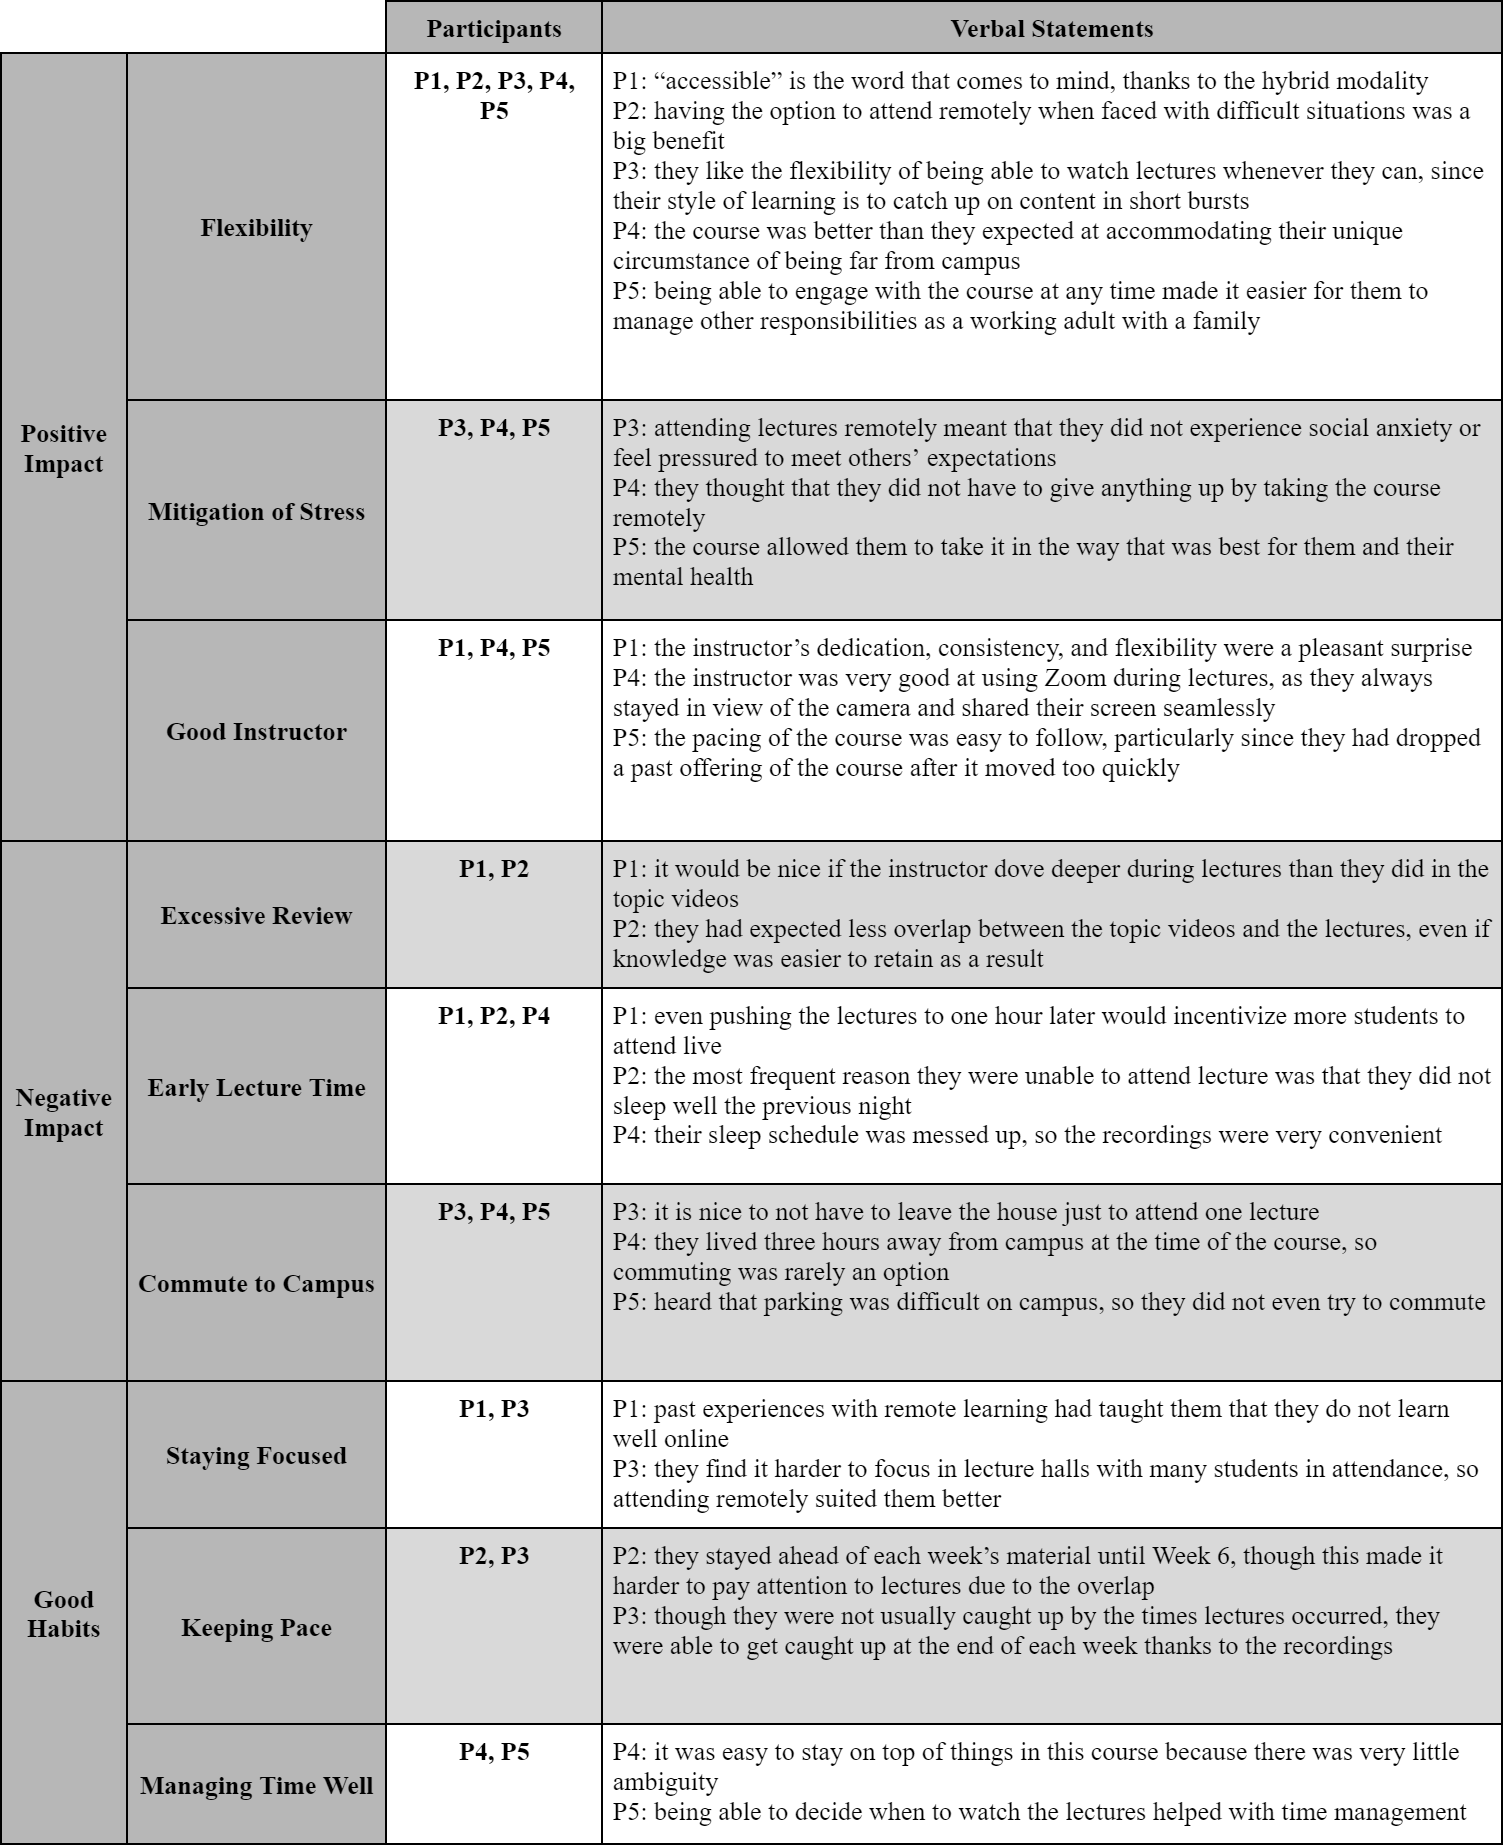
\includegraphics[width= 16cm]{figures/interview_response_codes.png}
    \label{tab:interview_response_codes}
\end{table}

\section{Identified Factors}

With the information that was provided to us by the interview participants and the responses that we gathered through the course surveys, we were able to identify the following five primary factors that impact the modality and frequency of a student’s lecture attendance in a flipped HyFlex course.

\subsection{Personal Preference}

99.0\% of pre-course survey respondents stated that they had used the remote conferencing tool Zoom in one of their previous courses, meaning that very few students had their first experience with remote learning at the time of the study. As a result, many students had already determined which modality they would prefer, in-person or remote, before they had even started the course. When asked which modality they would prefer if the course had been offered as solely in-person or solely remote, 39.0\% chose in-person, 39.7\% chose remote, and 21.3\% stated no preference either way. As shown in Table \ref{tab:attendance-initial-preference}, students who said that they would prefer an in-person course were much more likely to attend the lectures in person during the first half of the course. When P1 was asked why they preferred to learn in person, they explained that their fully remote senior year of high school had demonstrated to them that they are unable to engage properly with their schoolwork without “seeing it in front of [them] and having fewer distractions.” They always tried to attend the lectures live so that they could learn important information without having to watch the lecture recordings, which they rarely did out of dislike for the format. On the opposite end of the spectrum, P5’s discovery that they could engage with the lectures at any time throughout the week through the recordings was instrumental in their ability to succeed in the course; they mentioned that they had dropped the course in the past due to feeling unprepared for the pace at which they would need to learn.

\subsection{Early Expectations}

All five interviewees had entered the course with a general idea of how they would be attending each of the lectures. Of them, the in-person and hybrid attendees (P1 and P2) were let down by the in-person lecturing experience they received, while the remote and asynchronous attendees (P3, P4, and P5) found that the lectures surpassed their expectations for what a remote course could offer them. The differences in their expectations could be explained by the high standards that the students had for in-person courses and the relatively lower standard for remote courses that they had developed during the COVID-19 pandemic: P4 stated that several remote courses they had taken in the past had clearly been designed for in-person attendees, and they asserted that “some professors can’t teach online and provide a cohesive experience at the same time.” This course had been the first to show P4 that it could be achieved successfully at a large scale. And based on the survey data depicted in Table \ref{tab:attendance-initial-preference}, it appears that they were not alone in this regard: over half of the students who submitted responses to both the pre-course and the end-of-course surveys attended lectures asynchronously as they reached the end of the course, denoting a large shift away from the in-person end of the modality spectrum. Though most fully in-person courses in the department also regularly experience a drop-off in attendance over time, the way that this course was able to provide a comparable experience to remote, asynchronous, and non-attendees surprised students: when asked about the ways in which the course differed from their expectations in an optional question on the end-of-course survey, 7 of the 32 respondents took the opportunity to simply say that the hybrid model had far surpassed what they had anticipated. One student noted that they were “honestly surprised that this hybrid structure isn't the standard for courses in the department.”

\subsection{Conflicting Circumstances}

The interviewees who attended remotely or asynchronously each cited physical location as a reason why they would not be able to attend lectures in person: P3 stated that they enjoyed not having to leave their house just to attend the one lecture they had on Mondays, Wednesdays, and Fridays, while P4 and P5 both resided a long distance from campus and would not be able to attend without conducting a lengthy commute. Given that the course had been advertised beforehand as a hybrid course, these individuals had knowingly enrolled in the course with the intent to take advantage of the remote and asynchronous modalities from a distant location, limiting their available options from the very beginning. As can be seen in Figure \ref{fig:remote_attendance_reasons}, around 15\% of respondents to the mid-course and end-of-course survey cited physical distance from their on-campus residences as a reason for their inability to attend lectures in person, while a further 5\% stated that they resided off-campus and did not have a method of transportation to arrive at the location of the lectures. However, a much more common reason why students were unable to attend in person was the timing of the lectures: over half of the respondents to the mid-course survey cited the early lecture times as a factor in their decision to not attend in-person lectures, while just under half of the end-of-course survey respondents gave the same reasoning. The interviewees who had attended in-person lectures, P1 and P2, both spoke about how the earliness of the lectures had negatively impacted their ability to attend consistently, with the latter mentioning that their inconsistent sleep schedule occasionally made in-person attendance an impossibility. This would indicate that, while an inconvenient location rules out in-person attendance entirely for individuals who plan to take lectures from the start, inconvenient timing will drastically decrease the motivation to attend in-person lectures in those who would otherwise be able to do so.

\subsection{Flexible Format}

Despite the difference in the modalities that were experienced by each of the interviewees, all of them were similarly impacted by the flexibility afforded to them by the dual-modality structure of the course. P1 and P2 both attested that, despite their frequent in-person attendance, they were unconcerned about missing the occasional lecture because they were able to attend remotely or asynchronously through the lecture recordings. P3, P4, and P5 all claimed that having the ability to absorb the material at their own pace was beneficial to their time management for the course; P5, having developed self-discipline in their past as a member of the military, spoke highly about the level of control that the course granted them over their education and its removal of stresses unrelated to the course, such as the lengthy commute and the availability of on-campus parking. This sentiment was echoed in 17 of 24 responses to an optional question on the mid-course survey: commutes, early lectures, and the inability to find parking were the factors most frequently cited by students when they were asked to explain why they did not attend in person. When one can join a lecture at the press of a button or the click of a link, or watch a recording later on EdStem, it was difficult for them to justify waking up early and dealing with the hassle of their commute. As seen in Table \ref{tab:attendance-modalities-tab}, the percentage of students who attended lectures in person dropped from 28.5\% in the first half of the course to 16.8\% in the second half, and synchronous attendees collectively dropped from 48.6\% to 25.0\% during the same time frame.

\subsection{Insightful Instructor}

Another commonality among participants was their attestation that the expertise of the instructor motivated them to continue engaging with the lectures in some form or another. Both P1 and P4 were impressed by the instructor’s ability to split their attention across two different modalities at the same time, and they praised the level of familiarity that the instructor had with utilizing Zoom during lectures. P1, being an in-person attendee, observed that the instructor always made sure to verbally repeat their questions before answering them for the benefit of the remote attendees, and they felt that this prevented one of the main drawbacks of attending a lecture through Zoom that many other instructors are not even aware of. P4, being a remote attendee, noted that they could always see and hear the instructor because they kept within the camera frame and spoke directly into the microphone, a feat that they had never seen in a remote course before this one. Despite utilizing different modalities, both of these participants were able to notice these details, and both were incentivized to attend lectures more often as a result. Three respondents to an optional question on the end-of-course survey also took note of the instructor’s organizational and presentational skills, with one musing that they “wish [their] other professors could learn from this class.”

\vspace{2cm}